\chapter{Java3D}
En este apartado, se va a detallar el diagrama de clases del Motor 3D de animaciones, a través del cual se mostrarán los
aspectos estructurales de éste bloque funcional y las relaciones principales entre sus clases.\\

En primer lugar analizaremos las clases implicadas en este bloque funcional, describiendo los atributos y las operaciones 
de las mismas, y posteriormente describiremos las relaciones existentes entre las clases. Obviaremos la descripción de las
clases propias de la API Java3D.\\

   \section{Clases del motor 3D}

      \subsection{Clase SMGroup}
         \begin{table}[H]
            \centering
            \begin{tabular}{|p{4cm}|p{11.5cm}|}
            \hline
            \textbf{Nombre} & \textit{SMGroup.}\\ \hline
            \textbf{Descripción} & \textit{Esta clase hereda de la clase Group de la API de Java3D, y se trata de una clase
                                    que contiene un grupo de objetos y sus transformaciones, así como funciones para añadir
                                    interpolaciones a dichos objetos.}\\ \hline
            \textbf{Atributos} & \textit{\textbf{\_bounds}: Área a ser renderizada por el motor de Java3D.}\newline
                                 \textit{\textbf{\_rotation}: Rotación inicial del grupo de objetos.}\newline
                                 \textit{\textbf{\_translation}: Traslación inicial del grupo de objetos.}\newline
                                 \textit{\textbf{\_scale}: Escalado inicial del grupo de objetos.}\newline
                                 \textit{\textbf{\_child}: Nodo de objetos donde se añaden los hijos del grupo.}\\ \hline
            \end{tabular}
         \end{table}
         \begin{table}[h]
            \begin{tabular}{|p{4cm}|p{11.5cm}|}
            \hline
            \textbf{Operaciones} & \textit{\textbf{SMGroup}: Constructor. Crea un nuevo grupo con sus transformaciones.}\newline
                                    \textit{\textbf{addChild}: Añade un hijo al grupo.}\newline
                                    \textit{\textbf{translation}: Establece los parámetros de traslación iniciales del grupo.}\newline
                                    \textit{\textbf{rotation}: Establece los parámetros de rotación iniciales del grupo.}\newline
                                    \textit{\textbf{scale}: Establece los parámetros de escalado iniciales del grupo.}\newline
                                    \textit{\textbf{addRotationAnim}: añade un comportamiento SMRotationInterpolator al grupo.}\newline
                                    \textit{\textbf{addPositionAnim}: añade un comportamiento SMPositionInterpolator al grupo.}\\ \hline
            \end{tabular}
            \caption{Clase SMGroup.}
         \end{table}
         \begin{figure} [H] \begin{center}
            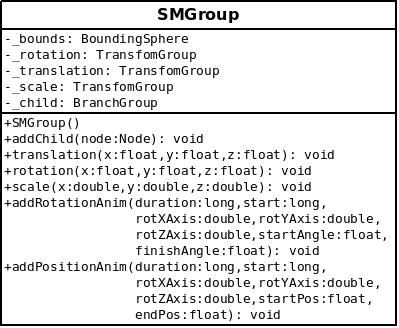
\includegraphics[width=0.9\textwidth]{./imagenes/SMGroup}\label{SMGroup}
            \caption{Clase: SMGroup.}
         \end{center} \end{figure}

      \subsection{Clase SMRotationInterpolator}
         \begin{table}[!ht] 
            \centering
            \begin{tabular}{|p{4cm}|p{11.5cm}|}
            \hline
            \textbf{Nombre} & \textit{SMRotationInterpolator.}\\ \hline
            \textbf{Descripción} & \textit{Esta clase hereda de la clase RotationInterpolator de la API Java3D. Se trata de un
                                    comportamiento de rotación que será aplicado sobre un grupo de transformación(TransformGroup
                                    de la API de Java3D) del cual será un nodo hijo.}\\ \hline
            \textbf{Atributos} & \textit{\textbf{\_start}: Tiempo de espera en milisegundos antes de comenzar la animación.}\newline
                                 \textit{\textbf{\_waitTime}: Tiempo de espera añadido al \_start en la creación del objeto.}\\ \hline
            \textbf{Operaciones} & \textit{\textbf{SMRotationInterpolator}: Constructor. Crea una nueva animación de rotación sobre un
                                          grupo de transformación.}\newline
                                    \textit{\textbf{initializate}: Establece el tiempo en el cual comienza la animación, y la hace efectiva.}\\ \hline
            \end{tabular}
            \caption{Clase SMRotationInterpolator.}
         \end{table}
         \begin{figure} [H] \begin{center}
            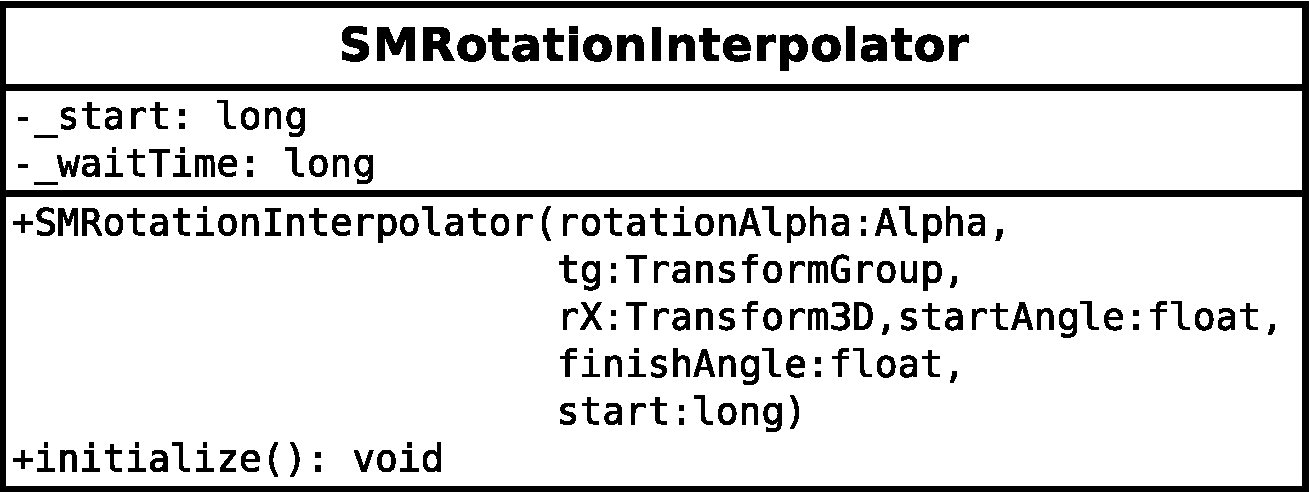
\includegraphics[width=0.9\textwidth]{./imagenes/SMRotationInterpolator}\label{SMRotationInterpolator}
            \caption{Clase: SMRotationInterpolator.}
         \end{center} \end{figure}

      \subsection{Clase SMPositionInterpolator}
         \begin{table}[!ht] 
            \centering
            \begin{tabular}{|p{4cm}|p{11.5cm}|}
            \hline
            \textbf{Nombre} & \textit{SMPositionInterpolator.}\\ \hline
            \textbf{Descripción} & \textit{Esta clase hereda de la clase PositionInterpolator de la API Java3D. Se trata de un
                                    comportamiento de traslación que será aplicado sobre un grupo de transformación(TransformGroup
                                    de la API de Java3D) del cual será un nodo hijo.}\\ \hline
            \textbf{Atributos} & \textit{\textbf{\_start}: Tiempo de espera en milisegundos antes de comenzar la animación..}\newline
                                 \textit{\textbf{\_waitTime}: Tiempo de espera añadido al \_start en la creación del objeto..}\\ \hline
            \textbf{Operaciones} & \textit{\textbf{SMPositionInterpolator}: Constructor. Crea una nueva animación de traslación sobre un 
                                    grupo de transformación..}\newline
                                    \textit{\textbf{initializate}: Establece el tiempo en el cual comienza la animación, y la hace 
                                    efectiva..}\\ \hline
            \end{tabular}
            \caption{Clase SMPositionInterpolator.}
         \end{table}
         \begin{figure} [H] \begin{center}
            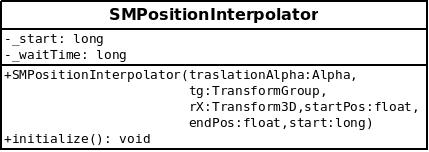
\includegraphics[width=0.9\textwidth]{./imagenes/SMPositionInterpolator}\label{SMPositionInterpolator}
            \caption{Clase SMPositionInterpolator.}
         \end{center} \end{figure}

      
      \subsection{Clase Stickman}
         \begin{table}[!ht] 
            \centering
            \begin{tabular}{|p{4cm}|p{11.5cm}|}
            \hline
            \textbf{Nombre} & \textit{Stickman.}\\ \hline
            \textbf{Descripción} & \textit{Esta clase hereda de SMGroup y se trata del cuerpo del Stickman.}\\ \hline
            \textbf{Atributos} & \textit{\textbf{BODYH}: Altura del cilindro que simula el cuerpo.}\newline
                                 \textit{\textbf{BODYR}: Radio del cilindro que simula el cuerpo.}\newline
                                 \textit{\textbf{rArmAngle}: Ángulo inicial que forma el cuerpo con el brazo derecho.}\newline
                                 \textit{\textbf{lArmAngle}: Ángulo inicial que forma el cuerpo con el brazo izquierdo.}\newline
                                 \textit{\textbf{rLegAngle}: Ángulo inicial que forma el cuerpo con la pierna derecha.}\newline
                                 \textit{\textbf{lLegAngle}: Ángulo inicial que forma el cuerpo con la pierna izquierda.}\newline
                                 \textit{\textbf{headAngle}: Ángulo inicial que forma el cuerpo con la cabeza.}\newline
                                 \textit{\textbf{rArm}: Brazo derecho.}\newline
                                 \textit{\textbf{lArm}: Brazo izquierdo.}\newline
                                 \textit{\textbf{rLeg}: Pierna derecha.}\newline
                                 \textit{\textbf{lLeg}: Pierna izquierda.}\newline
                                 \textit{\textbf{head}: Cabeza.}\\ \hline
            \textbf{Operaciones} & \textit{\textbf{Stickman}: Constructor. Crea el Stickman.}\newline
                                    \textit{\textbf{updateJoints}: Actualiza la posición y rotación de cada una de las extremidades
                                          del cuerpo del Stickman.}\\ \hline
            \end{tabular}
            \caption{Clase Stickman.}
         \end{table}
         \begin{figure} [H] \begin{center}
            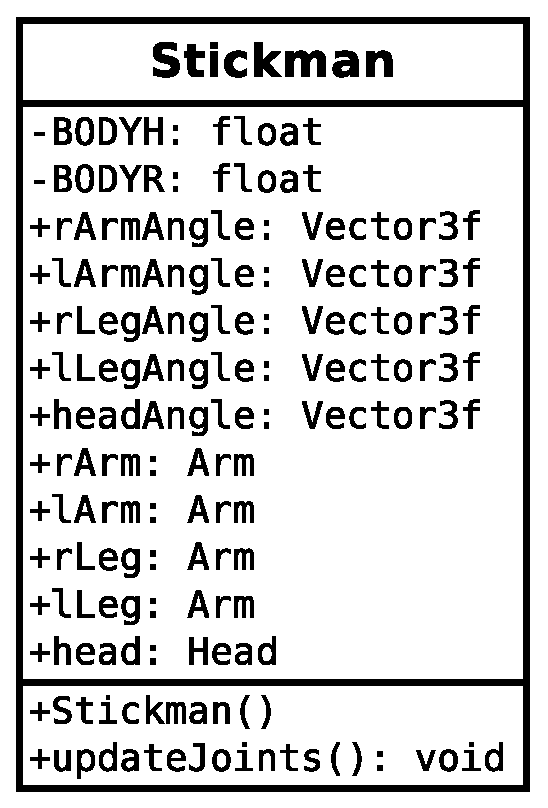
\includegraphics[width=0.9\textwidth]{./imagenes/Stickman}\label{Stickman}
            \caption{Clase Stickman.}
         \end{center} \end{figure}


      \subsection{Clase Arm}
         \begin{table}[!ht] 
            \centering
            \begin{tabular}{|p{4cm}|p{11.5cm}|}
            \hline
            \textbf{Nombre} & \textit{Arm.}\\ \hline
            \textbf{Descripción} & \textit{Esta clase hereda de la clase SMGroup y representa una extremidad del Stickman.}\\ \hline
            \textbf{Atributos} & \textit{\textbf{HEIGHT}: Altura del cilindro que simula la primera parte de la extremidad.}\newline
                                 \textit{\textbf{RADIUS}: Radio del cilindro que simula la primera parte de la extremidad.}\newline
                                 \textit{\textbf{foreAngle}: Ángulo que forma la segunda parte de la extremidad con la primera.}\newline
                                 \textit{\textbf{fore}: Segunda parte de la extremidad.}\\ \hline
            \textbf{Operaciones} & \textit{\textbf{Arm}: Constructor. Crea la extremidad.}\newline
                                    \textit{\textbf{updateJoint}: Actualiza la posición y rotación de la segunda parte de la extremidad.}\newline
                                    \textit{\textbf{setForeAngle}: Establece el ángulo que forma la segunda parte de la extremidad con la primera.}\\ \hline
            \end{tabular}
            \caption{Clase Arm.}
         \end{table}
         \begin{figure} [H] \begin{center}
            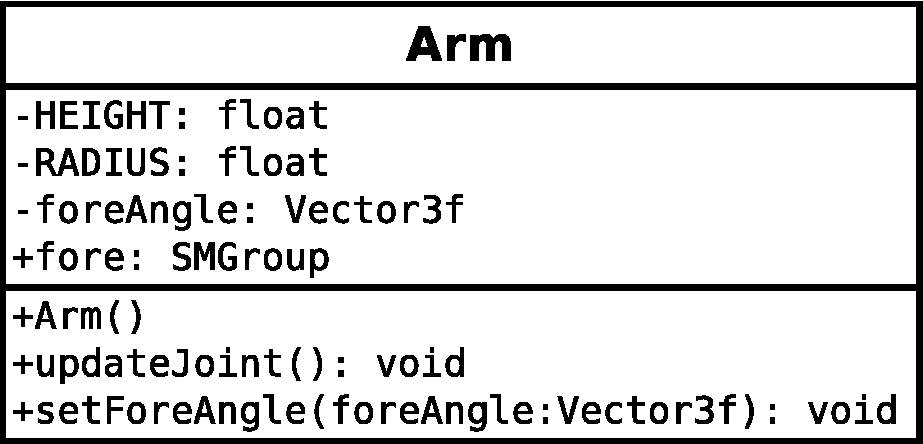
\includegraphics[width=0.9\textwidth]{./imagenes/Arm}\label{Arm}
            \caption{Clase Arm.}
         \end{center} \end{figure}

      \subsection{Clase Head}
         \begin{table}[!ht] 
            \centering
            \begin{tabular}{|p{4cm}|p{11.5cm}|}
            \hline
            \textbf{Nombre} & \textit{Head.}\\ \hline
            \textbf{Descripción} & \textit{Esta clase hereda de la clase SMGroup y representa a la cabeza del Stickman.}\\ \hline
            \textbf{Atributos} & \textit{\textbf{HEADSIZE}: Tamaño de la cabeza.}\newline
                                 \textit{\textbf{LENGTH}: Altura donde se posiciona la cabeza.}\newline
                                 \textit{\textbf{angle}: Ángulo que forma la cabeza.}\\ \hline
            \textbf{Operaciones} & \textit{\textbf{Head}: Constructor. Crea la cabeza.}\newline
                                    \textit{\textbf{rotation}: Establece la rotación de la cabeza.}\newline
                                    \textit{\textbf{translation}: Establece la posición de la cabeza.}\\ \hline
            \end{tabular}
            \caption{Clase Head.}
         \end{table}
         \begin{figure} [H] \begin{center}
            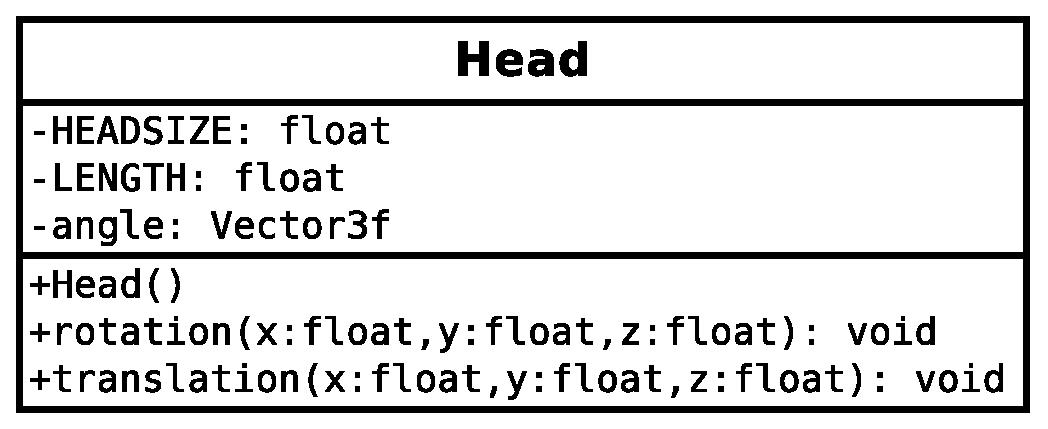
\includegraphics[width=0.9\textwidth]{./imagenes/Head}\label{Head}
            \caption{Clase Head.}
         \end{center} \end{figure}


      \subsection{Clase TransCylinder}
         \begin{table}[!ht] 
            \centering
            \begin{tabular}{|p{4cm}|p{11.5cm}|}
            \hline
            \textbf{Nombre} & \textit{TransCylinder.}\\ \hline
            \textbf{Descripción} & \textit{Esta clase hereda de la clase TransformGroup de la API de Java3D y representa
                                    un cilindro trasladado de tal forma que, según su eje de coordenadas, tiene el centro
                                    de uno de sus extremos en la posición (0,0,0).}\\ \hline
            \textbf{Atributos} & \\ \hline
            \textbf{Operaciones} & \textit{\textbf{TransCylinder}: Constructor. Crea el cilindro trasladado.}\\ \hline
            \end{tabular}
            \caption{Clase TransCylinder.}
         \end{table}
         \begin{figure} [H] \begin{center}
            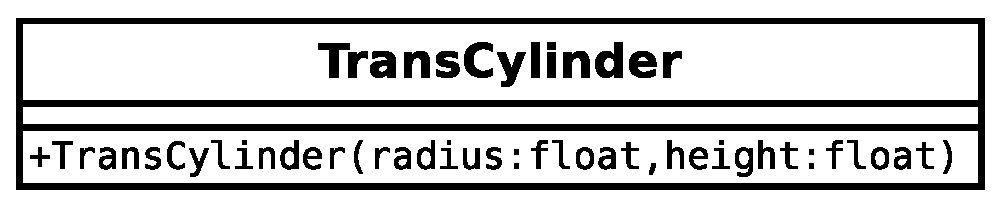
\includegraphics[width=0.9\textwidth]{./imagenes/TransCylinder}\label{TransCylinder}
            \caption{Clase TransCylinder.}
         \end{center} \end{figure}


      \subsection{Clase Scene}
         \begin{table}[!ht] 
            \centering
            \begin{tabular}{|p{4cm}|p{11.5cm}|}
            \hline
            \textbf{Nombre} & \textit{Scene.}\\ \hline
            \textbf{Descripción} & \textit{Esta clase es la encargada de crear toda la escena.}\\ \hline
            \textbf{Atributos} & \textit{\textbf{steve}: Stickman a mostrar.}\newline
                                 \textit{\textbf{time}: Tiempo actual de la escena.}\newline
                                 \textit{\textbf{sceneGroup}: Grupo que contiene a los elementos de la escena.}\newline
                                 \textit{\textbf{simpleU}: Universo en el cual se cargará la escena.}\newline
                                 \textit{\textbf{canvas3D}: Canvas donde el Universo será representado.}\\ \hline
            \textbf{Operaciones} & \textit{\textbf{Scene}: Constructor. Crea la escena.}\newline
                                    \textit{\textbf{Start}: Inicia la animación.}\newline
                                    \textit{\textbf{Reset}: Reinicia la animación.}\newline
                                    \textit{\textbf{createSceneGraph}: Crea los elementos que componen la escena.}\newline
                                    \textit{\textbf{getLigth}: Crea la luz de la escena.}\newline
                                    \textit{\textbf{rotateSMGroup}: Rota un SMGroup.}\newline
                                    \textit{\textbf{rotateHead}: Rota la cabeza del Stickman.}\newline
                                    \textit{\textbf{rotateRArm}: Rota el brazo derecho del Stickman.}\newline
                                    \textit{\textbf{rotateLArm}: Rota el brazo izquierdo del Stickman.}\newline
                                    \textit{\textbf{rotateRLeg}: Rota la pierna derecha del Stickman.}\newline
                                    \textit{\textbf{rotateLLeg}: Rota la pierna izquierda del Stickman.}\newline
                                    \textit{\textbf{flexRArm}: Flexiona el brazo derecho del Stickman.}\newline
                                    \textit{\textbf{flexLArm}: Flexiona el brazo izquierdo del Stickman.}\newline
                                    \textit{\textbf{flexRLeg}: Flexiona la pierna derecha del Stickman.}\newline
                                    \textit{\textbf{flexLLeg}: Flexiona la pierna izquierda del Stickman.}\newline
                                    \textit{\textbf{rotateStickman}: Rota el Stickman.}\newline
                                    \textit{\textbf{moveStickman}: Mueve el Stickman.}\newline
                                    \textit{\textbf{addTime}: Incrementa el tiempo de la escena.}\newline
                                    \textit{\textbf{getTime}: Devuelve el tiempo actual de la escena.}\newline
                                    \textit{\textbf{setTime}: Establece el tiempo actual de la escena.}\\ \hline
            \end{tabular}
            \caption{Clase Scene.}
         \end{table}
         \begin{figure} [H] \begin{center}
            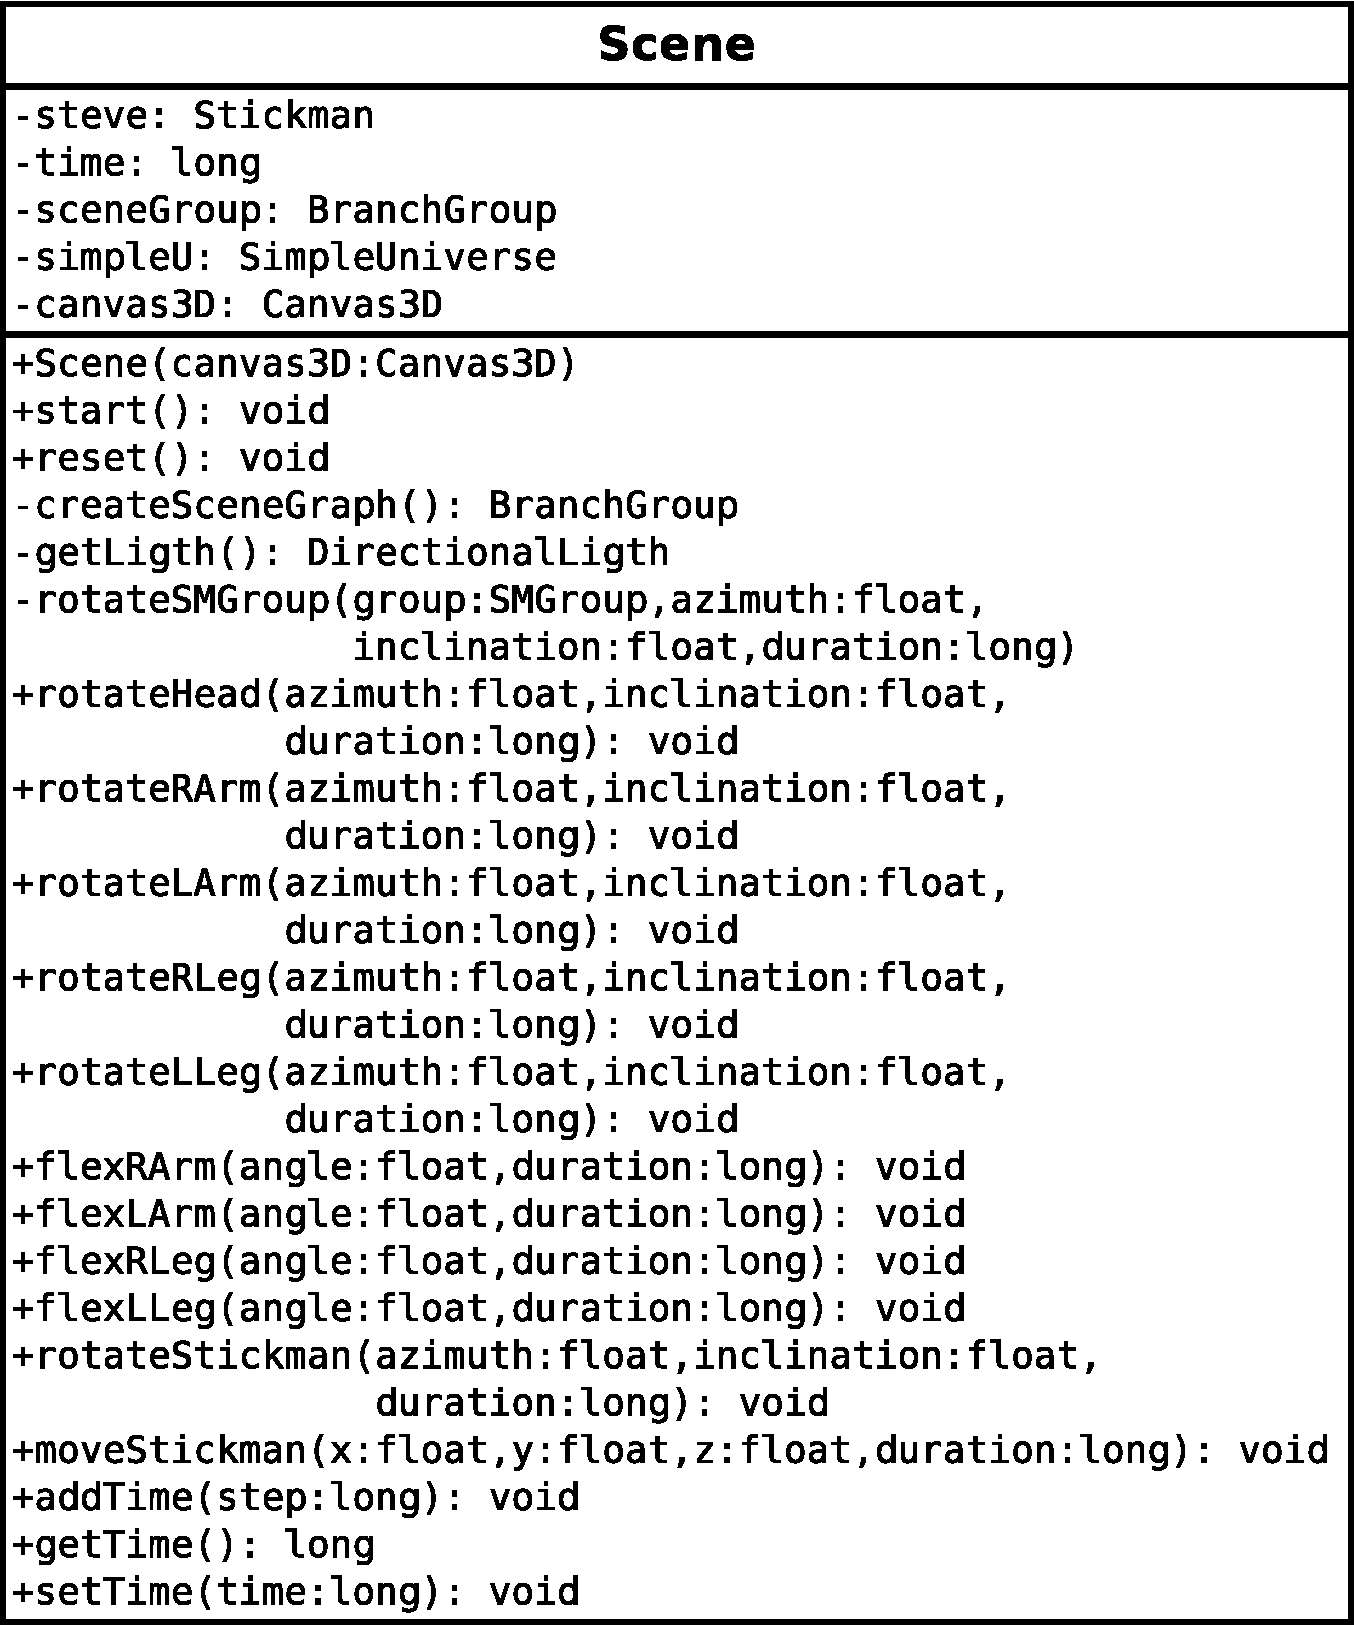
\includegraphics[width=0.9\textwidth]{./imagenes/Scene}\label{Scene}
            \caption{Clase Scene.}
         \end{center} \end{figure}

   \section{Descripción de las relaciones}
   Las clases anteriormente especificadas, junto a las propias de la API de Java3D, se relacionan de la siguiente forma:
   \begin{itemize}
      \item Scene-Stickman: Un Scene tiene un Stickman.
      \item Stickman-Head: Un Stickman tiene un Head.
      \item Stickman-Arm: Un Stickman tiene 4 Arms.
      \item Stickman-Cylinder: Un Stickman tiene un Cylinder.
      \item Stickman-SMGroup: Stickman es subclase de SMGroup.
      \item Arm-SMGroup: Arm es subclase de SMGroup.
      \item Arm-SMGroup: Arm tiene un SMGroup.
      \item Arm-TransCylinder: Un Arm tiene un TransCylinder.
      \item Head-SMGroup: Head es subclase de SMGroup.
      \item Head-ColorCube: Un Head tiene un ColorCube.
      \item TransCylinder-TransformGroup: TransCylinder es subclase de TransformGroup.
      \item SMGroup-Group: SMGroup es subclase de Group.
      \item SMGroup-TransformGroup: Un SMGroup tiene 3 o más TransformGroup.
      \item SMGroup-BranchGroup: Un SMGroup tiene un BranchGroup.
      \item SMGroup-BoundingSphere: Un SMGroup tiene un BoundingSphere.
      \item Group-Node: Group es subclase de Node.
      \item BranchGroup-Node: Un BranchGroup tiene 0 o muchos Node.
      \item TransformGroup-SMRotationInterpolator: Un TransformGroup tiene 0 o 1 SMRotationInterpolator.
      \item TransformGroup-SMPositionInterpolator: Un TransformGroup tiene 0 o 1 SMPositionInterpolator.
      \item SMRotationInterpolator-RotationInterpolator: SMRotationInterpolator es subclase de RotationInterpolator.
      \item SMPositionInterpolator-PositionInterpolator: SMPositionInterpolator es subclase de PositionInterpolator.
   \end{itemize}

   \section{Diagrama de clases}
   A continuación mostraremos el diagrama de clases. Este diagrama muestra aspectos estructurales acerca de las clases
   consideradas dentro del dominio de éste bloque funcional y de las relaciones principales necesarias entre las mismas 
   para cumplir con los requisitos funcionales correspondientes.
   \begin{figure} [H] \begin{center}
      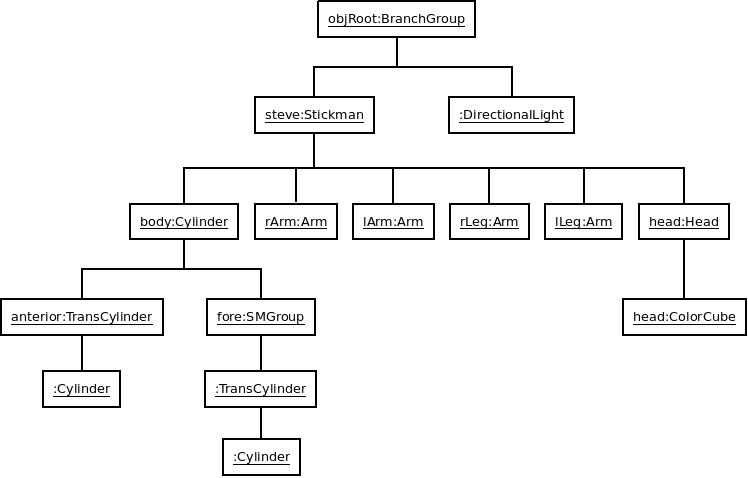
\includegraphics[width=0.9\textwidth]{./imagenes/engine3d}\label{engine3d}
      \caption{Diagrama de clases del bloque funcional motor 3D.}
   \end{center} \end{figure}


   \section{Diagrama de objetos}
   Debido a la complejidad que supone la creación de animaciones con Java3d, y una vez explicado todo el diseño estructural
   del motor 3d, hemos decidido mostrar, mediante un diagrama de objetos, cual sería el estado de los objetos y las relaciones
   entre sí que se llevan a cabo para crear la escena a mostrar.

   \begin{figure} [H] \begin{center}
      \includegraphics[width=0.9\textwidth]{./imagenes/engine3dObjetos}\label{engine3dObjetos}
      \caption{Diagrama de objetos del bloque funcional motor 3D.}
   \end{center} \end{figure}

   En el diagrama podemos observar el BranchGroup(grupo de objetos) que contiene la escena, el cual está compuesto del objeto 
   steve de la clase Stickmotion, que es el muñeco, y un objeto de la clase DirectionalLigth de la API de Java3D, que se trata
   de una luz direccional que hace visible la escena.\\

   El objeto steve, está compuesto de un cuerpo(body de la clase Cylinder de la API de Java3D, que es la geometría utilizada 
   para hacer de cuerpo del Stickman), 4 extremidades(rArm,lArm,rLeg y lLeg de la clase Arm) y una cabeza(head de la clase Head).\\

   El objeto head contiene a su vez un objeto head de la clase ColorCube de la API de Java3D que se trata de un cubo que hemos
   utilizado como geometría de la cabeza del Stickman.\\

   Los objetos de la clase Arm están compuestos a su vez de otros, como podemos observar en el siguiente diagrama de objetos.
   \begin{figure} [H] \begin{center}
      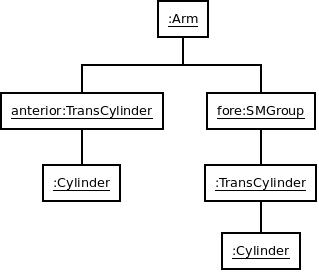
\includegraphics[width=0.9\textwidth]{./imagenes/arm}\label{arm}
      \caption{Diagrama de objetos de la clase Arm.}
   \end{center} \end{figure}

   Cada extremidad(objeto de la clase Arm) está compuesta por un anterior y un posterior(antebrazos y brazos o antepiernas y 
   piernas). Los anteriores son los objetos anterior de la clase TransCylinder, mientras que los posteriores son los objetos fore
   de la clase SMGroup.\\

   Un objeto anterior de la clase TransCylinder, tiene un objeto de la clase Cylinder de la API de Java3D, que es la geometría
   utilizada para representar el anterior de una extremidad.\\

   Un objeto fore de la clase SMGroup, tiene un objeto de la clase TransCylinder, que a su vez está compuesto de un objeto 
   Cylinder de la API de Java3D, que es la geometría utilizada para representar el posterior de una extremidad.\\

   Por último, es conveniente explicar como se crean las animaciones, por lo cual cabe destacar que todos los objetos que forman
   parte de un objeto de la clase Stickman, así como él mismo, son objetos de clases que heredan de la clase SMGroup, como ya se
   explicó anteriormente en la descripción de las clases.\\

   Para añadir una animación de alguna clase SMGroup, bastaría con asociar un comportamiento, es decir, un objeto de la clase
   SMRotationInterpolator o SMPositionInterpolator. Esto se hace a través de un objeto de la clase TransformGroup de la API de Java3D.\\

   En definitiva, por cada animación, se añade un objeto de la clase SMRotationInterpolator o de la clase SMPositionInterpolator
   a un objeto de la clase TransformGroup, y éste último se añade al árbol de objetos que posee el objeto de la clase SMGroup.\\

   Java3D funciona con árboles de objetos, por lo cual se debe tener en cuenta que cualquier tipo de transformación se realiza sobre los
   hijos que ésta transformación posee. Así mismo, cualquier nodo que no esté colgando del árbol de la escena no será tenido
   en cuenta por Java3D, es decir, no afectará a dicha escena.\\

   

